\chapter{Jets}\label{jets}


Las lluvias colimadas de partículas que se producen cuando los quarks y gluones se hadronizan, y sus respectivos depósitos de energía en el detector se reconstruyen como jets. Para definir un jet es necesario decidir como combinar las partículas que fueron producidas en la hadronización, y sus decaimientos subsiguientes. Algunas de estas decisiones involucradas en la \emph{definición} de un jet responden a preguntas como: cuando un quark radía un gluón, para qué rango cinemático debería el gluón ser parte del jet originado por el quark, o por el contrario, ser considerado como un jet aparte. En una visión simplificada, un jet se reconstruye de manera que sus propiedades (por ejemplo, momento transverso y dirección) se correspondan con un partón del hard scattering que pasó por un ``soft and colinear showering '' y una posterior hadronización (ver fig. \ref{fig:jetScheme}). Los jets también pueden formarse a partir de los productos de los decaimientos hadrónicos de partículas pesadas, por ejemplo, bosones W o Z o el quark top.

\begin{figure}[h]
    \centering
    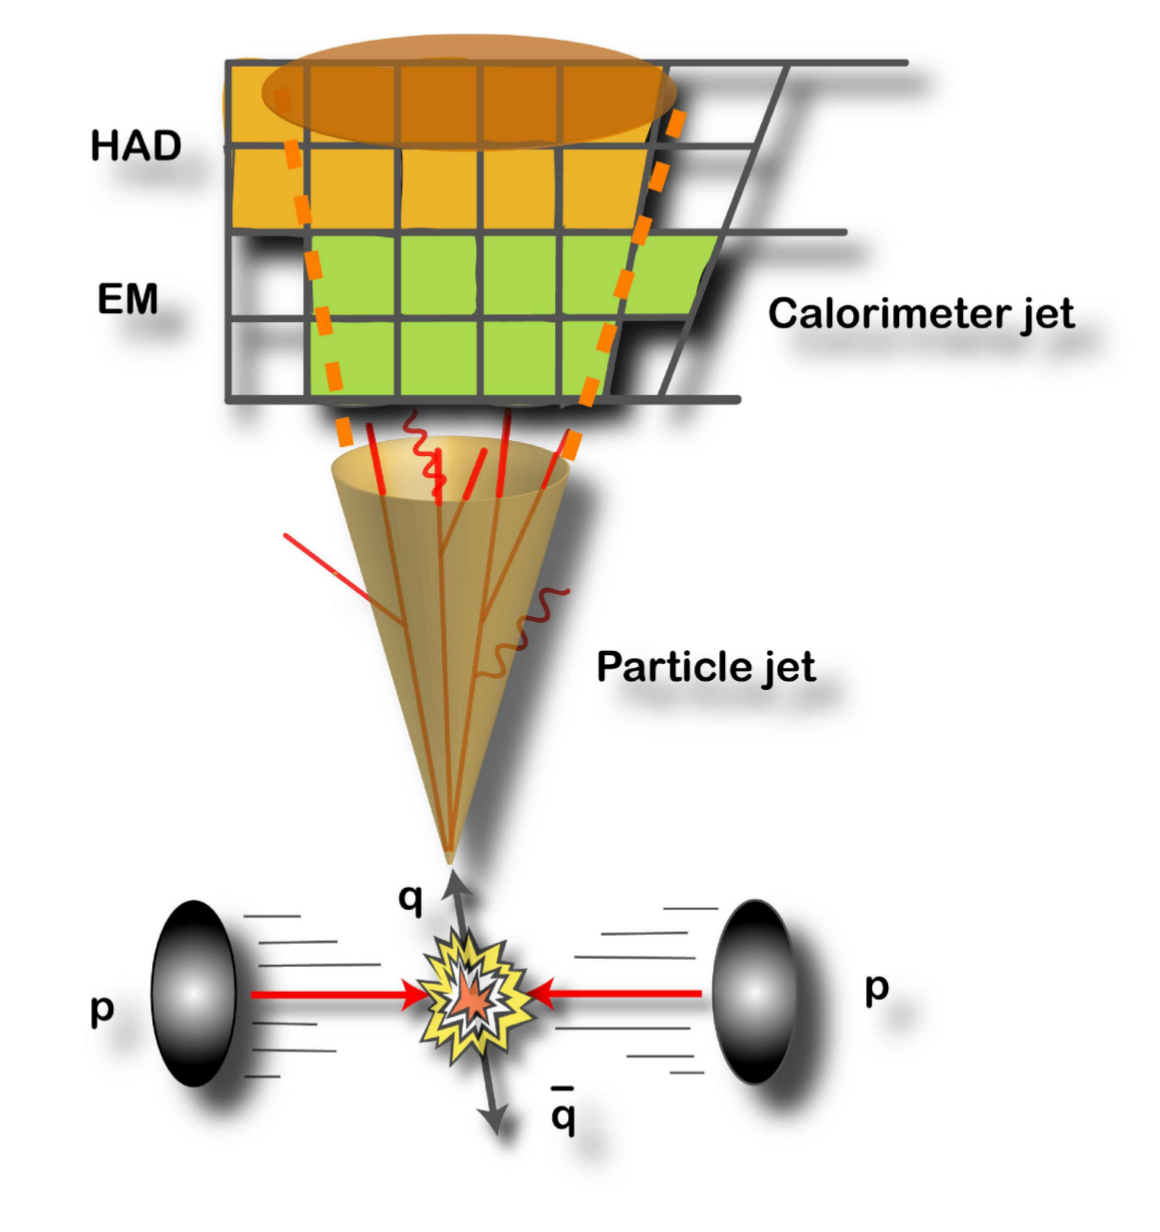
\includegraphics[width =0.6\linewidth]{images/jetScheme}
    \caption{Esquema de la producción de un jet. Se radía un partón el cual se hadroniza produciendo un jet de partículas. Este deposita energía en los calorímetros, y las señales detectadas se utilizan para recontruir jets calorimétricos.}
    \label{fig:jetScheme}
\end{figure}

Los algoritmos de reconstrucción de jets establecen un conjunto de reglas para agrupar partículas en jets. Generalmente, involucran uno o más parámetros que determinan cuan cerca deben estar dos partículas para pertenecer al mismo jet. Cualquier algoritmo formará un jet a partir de un único partón aislado; sin embargo, las diferentes definiciones de jets producirán resultados diferentes cuando, por ejemplo, hayan partones no aislados, o cuando un partón radie un gluón de poca energía. Un algoritmo de reconstrucción va acompañado de una estrategia de recombinación, que indica como combinar los cuadri-vectores de las partículas que conforman al jet. 

Una buena definición de jet debe ser \textit{infrared and collinear safe}, fácil de implementar tanto en un contexto teórico como en uno experimental, aplicable a cualquier tipo de inputs (momento de hadrones o partones, trazas de partículas cargadas, y depósitos de energia en el detector), y dar lugar a jets que no sean demasiado sensibles a efectos no perturbativos\cite{ParticleDataGroup}. 

Se le llama ``infrared and collinear safety'' (IRC Safety) a la propiedad de que si uno modifica un evento de manera de introducir una fragmentación colineal o una emisión de baja energía, el conjunto de jets que se reconstruyen en el evento no cambia (ver figura \ref{fig:IRC}). Uno de los motivos por los que se busca esta propiedad en una definición de jet tiene que ver con que, a orden fijo en cálculos de QCD perturbativo, las emisiones de baja energía y la fragmentación colineal están asociadas a divergencias que se cancelan; pero cuando el algoritmo no cuenta con esta propiedad, diagramas a un dado orden producen un conjunto de jets y a otro orden producen otro conjunto de jets, rompiendo con la cancelación y dando por resultado secciones eficaces que divergen en teoría de perturbaciones\cite{Jetography}\cite{RunIIJet}. 

\begin{figure}[h]
    \centering
    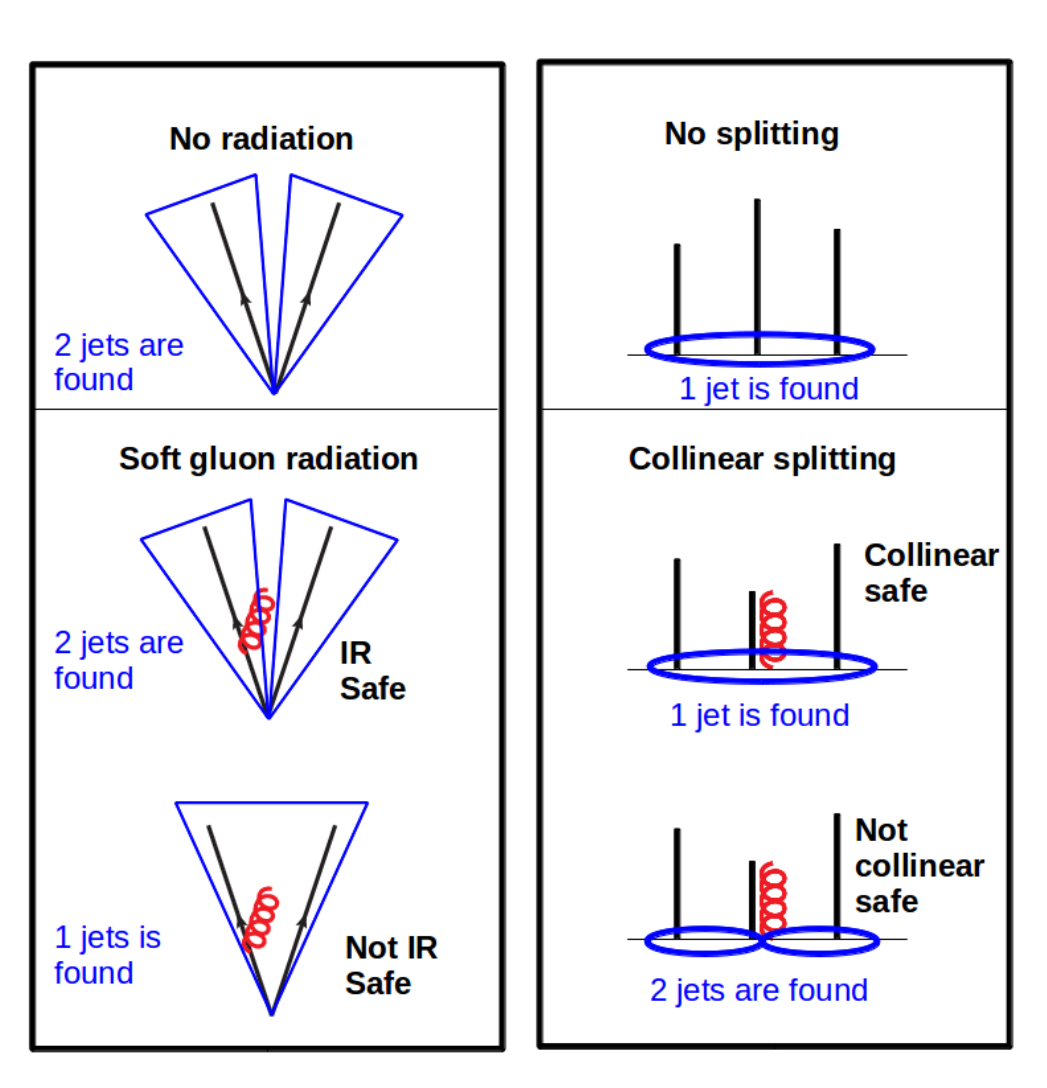
\includegraphics[width =0.6\linewidth]{images/IRC}
    \caption{\emph{Infrared and collineal safety (IRC Safety)}. La figura de la izquierda muestra como dos partones (sin radiación) dan lugar a dos jets. Si el algoritmo es IRC Safe, la recontrucción de jets no se verá afectada por la emisión de un gluón de baja energía (diagrama de en medio), mientras que si no lo es, la recontrucción dará por resultado un único jet donde antes había dos (diagrama inferior). En la figura de la derecha se muestra (arriba) la recontrucción de un jet asociado a tres partones. Si el método es IRC Safe, la recontrucción de jets no se verá afectada por la fragmentación de un partón (medio), mientras que si no lo es, la reconstrucción dará por resultado dos jets donde antes había uno (abajo).}
    \label{fig:IRC}
\end{figure}

\section{Algoritmos de Reconstrucción de Jets}\label{JetAlgo}
Existen varios algoritmos de reconstrucción de jets y estrategias de recombinación, un \emph{review} más completo puede encontrarse en la referencia \cite{Jetography}. Los algoritmos de reconstrucción de jets pueden dividirse en dos categorías: algoritmos cónicos y algoritmos de recombinación secuencial. A grandes rasgos, la mayoría de los algoritmos cónicos comienzan con alguna partícula semilla, suman el momento de todas las partículas dentro de una apertura angular R (parámetro a determinar), típicamente definido en términos del ángulo $\varphi$ y la (pseudo-)rapidez. Luego se toma la dirección de esta suma como nueva semilla y se repite el proceso hasta que el cono resulta estable, y se denomina al contenido del cono resultante como jet si su momento transverso queda por encima de un umbral. 

Las definiciones de Jets que se usan en ATLAS son algoritmos de recombinación secuencial que cumplen con la propiedad de IRC. Estos algoritmos hacen uso de dos distancias: la distancia $d_{ij} = min(p_{t,i}^{2p},p_{t,j}^{2p}) \Delta R_{ij}^2 / R^2$ entre todos los pares de partículas\footnote{También aplicable a otros inputs, como por ejemplo $clusters$. En este caso, la distancia $d_{ij}$ hace referencia a una distancia cluster-cluster, mientras que la distancia $d_{iB}$ hace referencia a la distancia cluster-haz.} \emph{i,j}, donde $ \Delta R_{ij}$ es su separación en el plano ($\varphi, y$), $p_{t,i}$ es el momento transverso (según el haz incidente), y $R$ es un parámetro libre; y la distancia calculada $d_{iB}=p_{t,i}^2$, que hace referencia a la distancia al haz. Luego se toma la menor de las dos distancias para todos los $d_{ij}$ y los $d_{iB}$, y si ésta resulta ser de la forma $d_{ij}$ entonces las partículas $i$ y $j$ se combinan en una nueva pseudo-partícula, siguiendo la estrategia de recombinación, y se vuelve a repetir el procedimiento. Si la mínima distancia es de la forma $d_{iB}$, entonces la partícula $i$ se remueve de la lista de partículas y se la declara un jet. El proceso se repite hasta que no queden partículas. Al igual que con los algoritmos cónicos, sólo se catalogan como jets aquellos que estén por encima de un dado umbral de momento transverso\cite{ParticleDataGroup}. 

El parámetro $p$ del algoritmo determina el orden en que las partículas en un evento se combinan y por lo tanto afecta la forma final del jet. El valor $p=1$ corresponde al $(inclusive-)k_t$ $algorithm$, $p=0$ corresponde al $Cambridge-Achen$ $algorithm$ , y para $p=-1$ se tiene el $anti-k_t$ $algorithm$ \cite{Jetography}\cite{antiKtalgo}. Todas estas variantes son IRC safe a todo orden en teoría de perturbaciones. El algoritmo $anti-k_t$ favorece agrupamientos o $clusterings$ de partículas energéticas en vez de clusterings de partículas ``soft'' (algoritmo $k_t$) o clusterings independientes de la energía (algortimo Cambdrige-Achen). De esta manera, el algoritmo $anti-k_t$ forma jets que crecen hacia afuera alrededor de semillas energéticas, resultando en jets de forma circular. En la figura \ref{fig:algos} se muestran los jets formados por estos tres algoritmos, para el mismo evento a nivel partónico y el mismo parámetro $R$. Debido a que la forma del jet $anti-k_t$ en el espacio $y-\varphi$ varía poco al agregar radiación de poca energía, el algoritmo $anti-k_t$ es el elegido en experimentos como ATLAS.


\begin{figure}[h]
    \centering
    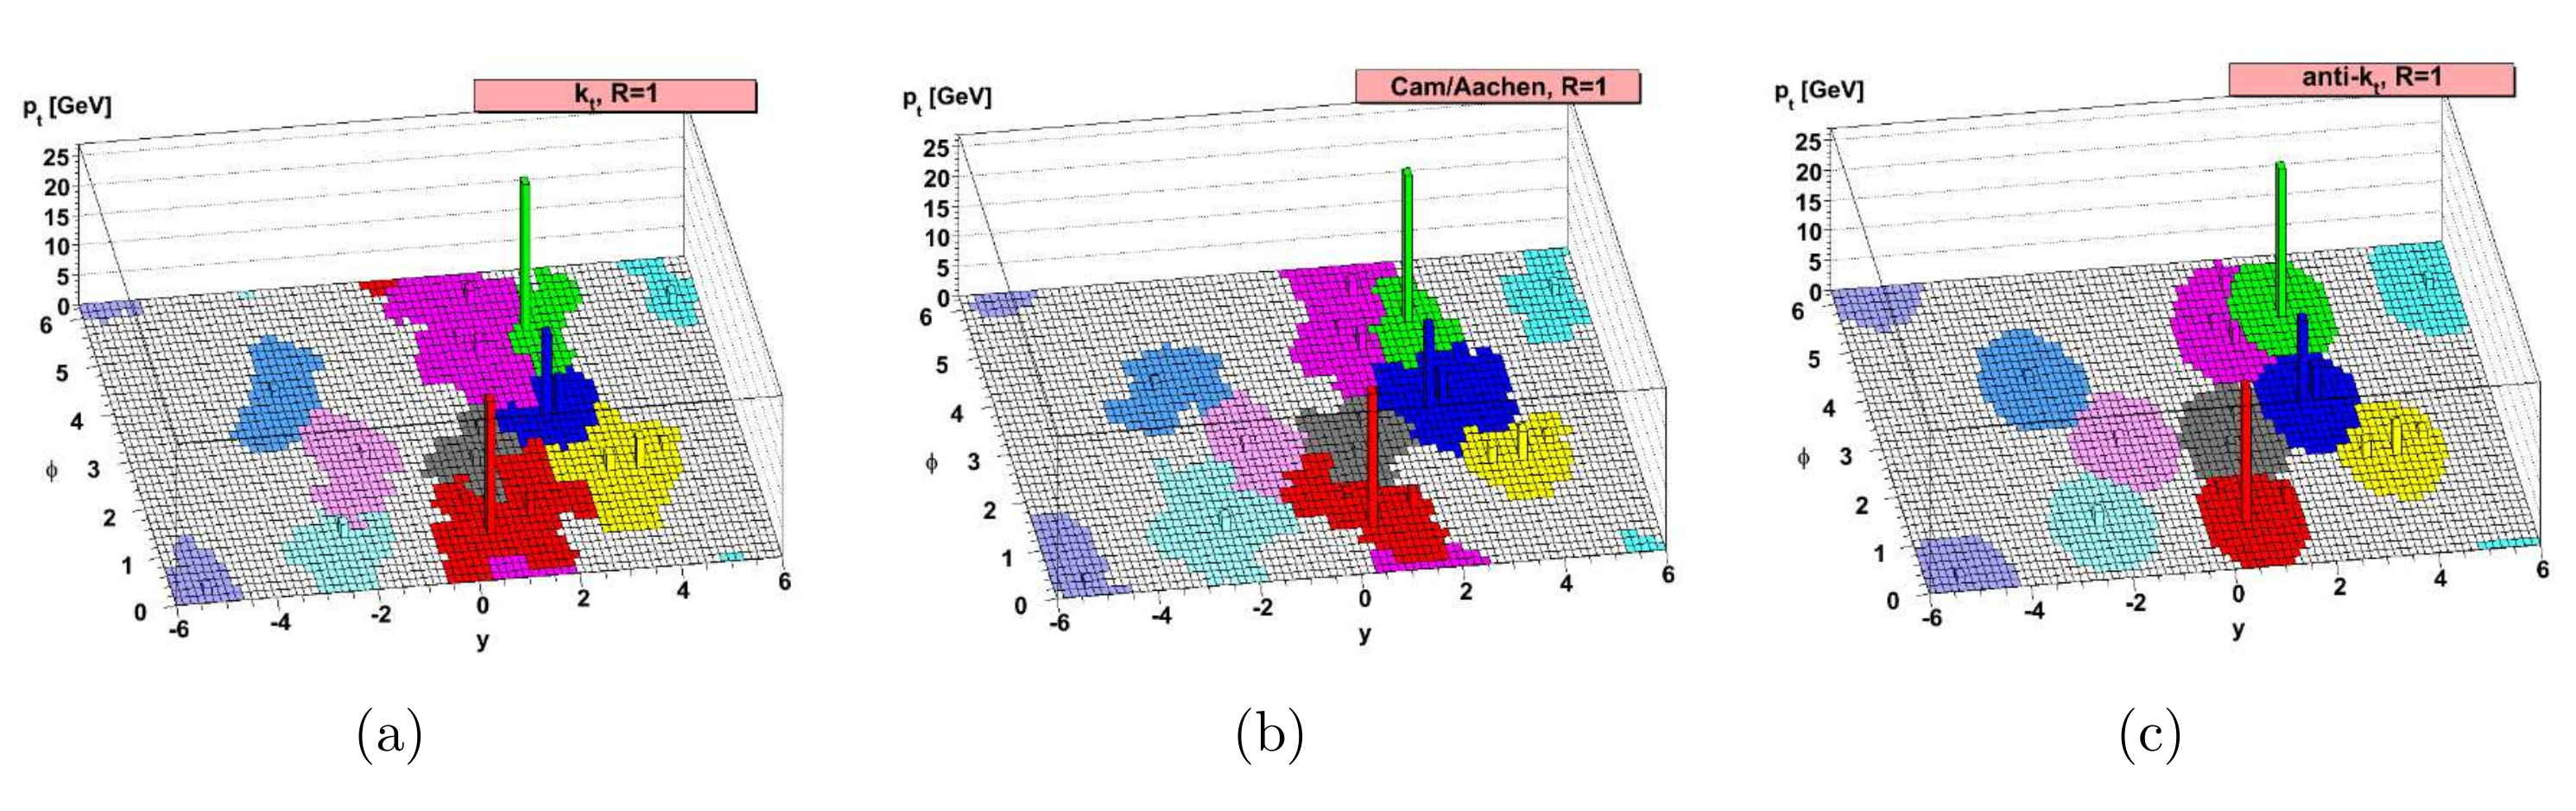
\includegraphics[width =\linewidth]{images/algos}
    \caption{ Los diagramas representan los jets formados en el espacio $\varphi$-$y$ por los algoritmos a)$k_t$, b)Cambirdge-Achen, c) $anti-k_t$ para un mismo evento a nivel partónico. Todos los jets tienen el mismo parámetro de distancia $R=1$\cite{antiKtalgo}. Las barras representan a los constituyentes a partir de los cuales se formaron los jets, su altura es proporcional a su momento transverso y el color indica a que jet corresponde. Para el algoritmo $anti-k_t$, los jets energéticos son, generalmente, de forma circular de radio $R$. }
    \label{fig:algos}
\end{figure}


\section{Jet Inputs} \label{JetInputs}
Para que se pueda ejecutar un algoritmo de reconstrucción de jets, se necesita una lista de objetos que sirvan como inputs en el proceso de ``clustering''. Idealmente, se tomaría como input a las partículas del estado final de una interacción. En eventos simulados, efectivamente se tiene acceso a esta información y los jets se construyen a partir de las partículas producto de la hadronización (y sus subsiguientes decaimientos) con vida media lo suficientemente larga como para ser detectada. Estos jets se conocen como \textit{truth jets}. 

En cambio, para colisiones reales, solamente se tiene acceso a trazas o depósitos de energía en los calorímetros. Así, se pueden utilizar las trazas reconstruidas de las partículas, ya sea en datos reales o en eventos simulados, para construir los denominados \textit{track jets}. 
En esta tesis se trabajó con jets reconstruidos, también conocidos como \textit{calorimeter/calo jets o reco jets}. Estos jets se construyen usando \textit{topological clusters} como inputs, ya sea en datos o en muestras de MC propagadas a través de la simulación del detector y simulando también la adquisición de la señal. 
Estos \textit{topological clusters} (o topo-clusters) son el resultado de combinar celdas calorimétricas tridimensionalmente según la energía que se haya depositado en ellas. La estrategia que se usa para combinar las celdas está diseñada para suprimir a las celdas calorimétricas que están dominadas por ruido, ya sea de tipo electrónico o pile-up. Esto se consigue considerando el cociente señal a ruido de las celdas, $E/\sigma$, donde $E$ es la energía medida en la celda calorimétrica y el ruido estimado es $\sigma=\sqrt{\sigma_{electronics}^2 + \sigma_{pile-up}^2}$. Para determinar $\sigma_{electronics}$ se mide la señal en los calorímetros cuando no hay colisiones; y  $\sigma_{pile-up}$ se determina a partir de mediciones de eventos de \textit{minimum-bias}\footnote{Eventos de scattering inelástico entre hadrones seleccionados con un trigger que se active con mínima actividad en el detector, pensados para seleccionar colisiones inelásticas con el menor \textit{bias} posible. Es decir, eventos seleccionados con la menor cantidad de requerimientos necesarios para asegurar que una colisión inelástica tuvo lugar. Estos eventos generalmente están asociados con eventos ``non-single diffractive''. Típicamente estos eventos están dominados por interacciones (``soft'') con momento transverso chico y una multiplicidad de partículas baja.}. Usando estas mediciones de ruido, la secuencia de clustering comienza encontrando una celda semilla con $E/\sigma>4$. Luego se agregan las celdas de alrededor, en las tres dimensiones, que verifican $E/\sigma>2$ y finalmente se agrega una capa de celdas con $E/\sigma\gtrsim0$. Una vez que se formaron todos los clusters, se utiliza un algoritmo de ``splitting'' para dividir a los topo-clusters que posean más de un máximo local de energía en clusters más pequeños. Una descripción más rigurosa del algoritmo de clustering se puede leer de la referencia \cite{TopoCluster}. 


\section{Calibración de Jets}\label{JetCalib}

La calibración de la escala de energía de los jets o JES (\textit{Jet energy scale}) es fundamental para relacionar las señales calorimétricas medidas con la energía que depositan las partículas en el detector y así poder reconstruir la energía y el momento de los (calo-)jets. Poder reconstruir la energía de los jets de manera precisa es de suma importancia en muchos análisis físicos en ATLAS, como por ejemplo en la medición de la sección eficaz inclusiva de producción de jets, la masa del quark top, o en la determinación del faltante de energía transversa, el cual juega un papel decisivo en muchas de las búsquedas de nueva física en ATLAS.

La calibración comienza con una calibración preliminar de los topo-clusters, convirtiendo la señal del detector en energía usando la escala electromagnética (EM). La escala EM describe correctamente la energía depositada en los calorímetros por una lluvia electromagnética. Esta escala de energía se establece mirando la respuesta de una porción del calorímetro a un haz de prueba (electrones, piones, fotones, muones o protones) de energía conocida. Comparando la señal en el calorímetro con la energía del haz incidente se mide la respuesta del calorímetro y entonces se puede determinar una calibración. Aún así, una calibración posterior es necesaria para corregir varios efectos del detector que afectan la medición de la energía del jet. Entre ellos se puede mencionar el hecho de que los calorímetros sean no-compensadores (ya discutido en la sección \ref{Lluvias}), posibles pérdidas de energía en zonas del detector no-instrumentadas (también llamadas \textit{material muerto}), partículas que traspasan el calorímetro y por lo tanto no pueden ser correctamente reconstruídas, o efectos del proceso de reconstrucción del jet \cite{Performance}. 

Otra posible calibración del topo-cluster es la llamada calibración local hadrónica o LCW (\textit{local cell weighting}) cuyo objetivo es el de proveer al algoritmo de reconstrucción de jets de clusters calibrados a una energía correspondiente a energías de partículas estables. Comienza por clasificar los topo-clusters (previamente calibrados a escala EM) en electromagnéticos o hadrónicos, llevando a una separación entre electrones, fotones y piones neutros, y hadrones cargados (mayormente piones) y neutrones. Si la clasificación resulta de tipo electromagnética, el topo-cluster queda calibrado a la escala EM. En cambio, en aquellos que fueron etiquetados como hadrónicos se procede a pesar sus celdas con la intención de compensar la respuesta del calorímetro a depósitos hadrónicos. Luego se aplican correcciones ``out-of-cluster'' por energía depositada en celdas calorimétricas en la cola de la lluvia hadrónica que quedan fuera de los clusters reconstruidos. Por último, se aplican correcciones para dar cuenta de la energía depositada en el material muerto (por ejemplo, cables, crióstatos y espacios entre módulos calorimétricos). Cada corrección se basa en simulaciones detalladas en $GEANT4$ haciendo uso de ``hits'' de calibración, es decir, accediendo a información de los distintos tipos de depósitos de energía ya sea en material activo como inactivo, y dando cuenta de la energía invisible (la energía liberada en procesos no-ionizantes como la ruptura de ligaduras nucleares) y la energía que se escapa del volumen del detector (debido a neutrinos o muones por ejemplo)\cite{LocalHadronic}.\\

\begin{figure}[h]
    \centering
    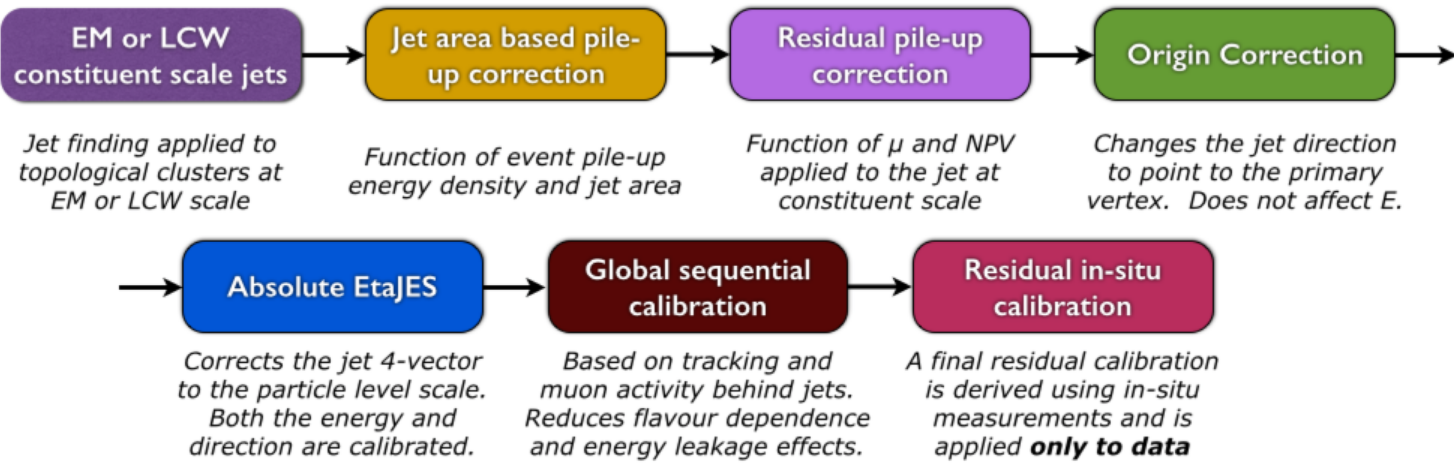
\includegraphics[width =\linewidth]{images/JES}
    \caption{ Overview de la calibración de jets en ATLAS \cite{JESpaper} }
    \label{fig:JES}
\end{figure}

Terminada la calibración de los topo-clusters, ya sea a escala EM o LCW, los jets en ATLAS se reconstruyen usando el algoritmo anti-$k_t$ con parámetro $R=0.4$
y se calibran siguiendo el esquema presentado en la figura \ref{fig:JES}\cite{JESpaper}. El objetivo de estas calibraciones es llevar la energía del jet reconstruido a la del \textit{truth jet} (ver sección \ref{JetInputs}).

El primer paso es suprimir la contribución de \textit{pile-up}. El pile-up puede afectar tanto la multiplicidad de los jets, la cual aumenta debido a la presencia de jets ``falsos'' provenientes de vértices de pile-up, como la energía del jet de interés, ya que la energía depositada en las celdas de los topo-clusters usados para construir el jet puede tener contribuciones no sólo del hard-scatter sino también de pile-up. Esta corrección (jet-a-jet y evento-a-evento) se realiza en dos etapas, la primera tiene en cuenta el área del jet en el espacio ($y,\varphi$) y la densidad de $p_t$ del pile-up, $\rho$ \cite{PileUpArea}; y la segunda es una corrección residual parametrizada en términos de $N_{PV}$, el número de vértices primarios\footnote{Los vértices primarios son aquellos vértices reconstruidos con un algoritmo iterativo \cite{NPV} a partir de las trayectorias de las partículas cargadas reconstruidas en base a las trazas detectadas en el ID.} en un bunch crossing (representativo del in-time pile-up), y de $<\mu>$, el número medio de interacciones por bunch crossing (representativo del out-of-time pile-up).

El siguiente paso de calibración corrige la dirección del jet de manera que éste apunte al vértice de interacción en vez de al centro nominal del detector ATLAS, manteniendo la energía constante. El vértice de interacción se determina tomando aquel que tiene el máximo valor de $\sum (p_t^{track})^2$, donde la suma se realiza sobre todas las trazas asociadas al vértice.

La siguiente corrección, conocida como la \textit{MC-JES} o \textit{Absolute Eta JES}, es la más significativa en la cadena y corrige el cuadri-momento del jet, llevándolo de la escala EM o LCW a la escala de energía de partículas, referida como \textit{EM+JES} o \textit{LC+JES}. La calibración de la energía y pseudo-rapidez del jet reconstruido se deriva completamente de simulaciones MC, donde los reco-jets se identifican angularmente (tomando $\Delta R<$0.33) con truth-jets. A partir de allí, se generan distribuciones de $E_{reco}/E_{truth}$ bineados tanto en $E_{truth}$ como en $|\eta_{det}|$ (medido desde el centro nominal del detector para poder distinguir claramente cuál es la región del detector responsable de la medición del jet). Entonces, para un dado jet, se busca el correspondiente bin y la corrección, en promedio, se obtiene de tomar la inversa de la media de esta distribución. 

La calibración continúa con la llamada \textit{Global Sequential Calibration} o GSC la cual se enfoca en reducir las diferencias en respuesta de jets iniciados por quarks livianos de los jets iniciados por gluones \footnote{Los jets iniciados por quarks generalmente incluyen hadrones con una fracción mayor del $p_t$ del jet y recorren más distancia sobre el calorímetro. Por otro lado, los jets iniciados por gluones típicamente se consituyen de partículas con $p_t$ menores, dando por resultado una respuesta calorimétrica menor y un perfil transverso mayor.}. 

Finalmente, se aplica una calibración residual \textit{in-situ} que aprovecha el balance de momento transverso del jet con algún objeto de referencia bien-medido (fotones, Zs y jets bien calibrados) para calibrar jets en datos. Esta calibración reduce el impacto de un modelado no del todo preciso por parte de las simulaciones MC, por ejemplo, en la descripción de la respuesta del detector o en la forma en la que se desarrollan las lluvias.\\

La incerteza asociada a la calibración de jets se deriva como función de $p_t$ y $|\eta_{det}|$. La componente principal proviene del uso de una simulación de MC y la necesidad de dar cuenta de los distintos modelados usados en distintos generadores de MC. Esta componente se deriva de comparar los resultados obtenidos usando diferentes generadores. La incerteza sistemática total se obtiene como la suma en cuadratura de diversas componentes, y tiene una fuerte dependencia en $\eta$. En la referencia \cite{JESpaper} se presenta la última calibración de jets disponible, reconstruidos con el algoritmo anti-$k_t$ con $R=$0.4 a partir de topo-clusters calibrados a la escala EM. Esta calibración se derivó a partir de los datos recolectados en el año 2015 en ATLAS, correspondiente a colisiones $pp$ a una energía de centro de masa de 13TeV con una luminosidad integrada de 3.2$fb^{-1}$. En la referencia se detallan los pasos de la calibración y sus resultados, y se determina la incerteza total de la misma, listando también todas las componentes sistemáticas y estadísticas consideradas.


